\chapter{Introduction}\label{chap:introduction}

\section{Sustainability}\label{sec:sustainability}
In 2015, the notion of \gls{sustainability} was defined by a set of 17 distinct goals by the UN.\cite{UN_sustain}. An overview of these goals is depicted in figure \ref{fig:sustainGoals}. Each goal was defined by a subset of different targets, aiming to define a successful completion of this goal. To evaluate the contribution of this work, the chosen research subject is mapped to specific goals and the concrete targets in section \ref{subsec:sustainabilityGoals}. The tangible legal frameworks, that are implemented in Germany are discussed in section \ref{subsec:nationalGoals}.

\begin{figure}
	\centering
	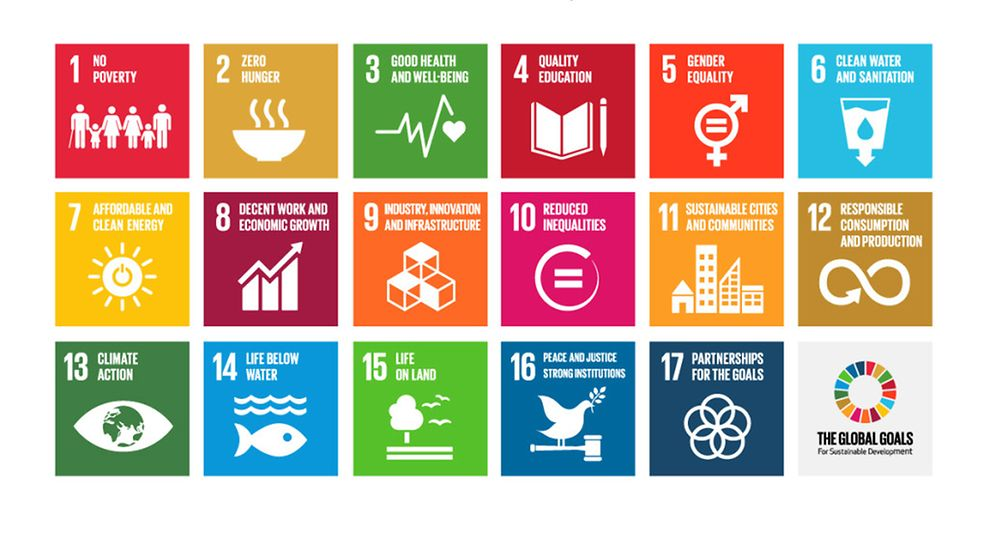
\includegraphics[width=\linewidth]{images/kacheln-the-global-goals.jpg}
	\caption{Overview of sustainability goals, adapted from The 2030 Agenda by Bundesregierung Deutschland, 2022 via https://www.bundesregierung.de/breg-en/issues/sustainability/global-goals-for-sustainable-development-355956}
	\label{fig:sustainGoals}
\end{figure}


\subsection{Sustainability Targets}\label{subsec:sustainabilityGoals}
\begin{figure}
        \centering
        \subgraphics{GOAL_7_TARGET_7.3.png}{}
        \subgraphics{GOAL_9_TARGET_9.C.png}{}
        \subgraphics{GOAL_11_TARGET_11.6.png}{}
        \subgraphics{GOAL_12_TARGET_12.6.png}{}
        \subgraphics{GOAL_12_TARGET_12.8.png}{}
        \subgraphics{GOAL_13_TARGET_13.3.png}{}
        \caption{Collection of targets concerned by energy efficiency adapted from Global Goals, 2022 via https://www.globalgoals.org/resources/}
        \label{fig:targets}
\end{figure}  

\subsection{National Goal Implementations}\label{subsec:nationalGoals}

\section{Power Consumption as a Contributor}\label{sec:powerConsumption}

\section{Related Work}\label{sec:relatedWork}

As expected by the expansive number of factors contributing to sustainability, the amount of related works is also numerous. The spectrum of different research questions reflect the many facets of the broad topic of sustainability
In \cite{10.1145/3136014.3136031} by Pereira et al. the power consumption of 26 different programming languages was compared on a small collection of standard problems. The results show a clear superiority of compiled languages compared to interpreted languages in terms of energy efficiency. Although not in every case, the efficiency with respect to time performance correlate very closely to total power consumption.